\documentclass[a4paper, 11pt]{article}
\newcommand\independent{\protect\mathpalette{\protect\independenT}{\perp}}
\def\independenT#1#2{\mathrel{\rlap{$#1#2$}\mkern4mu{#1#2}}}
\usepackage{comment} % enables the use of multi-line comments (\ifx \fi) 
\usepackage{lipsum} %This package just generates Lorem Ipsum filler text. 
\usepackage{fullpage} % changes the margin
\usepackage{tabularx}
\usepackage[a4paper, total={7in, 10in}]{geometry}
\usepackage[fleqn]{amsmath}
\usepackage{amssymb,amsthm}  % assumes amsmath package installed
\newtheorem{theorem}{Theorem}
\newtheorem{corollary}{Corollary}
\usepackage{graphicx}
\usepackage{tikz}
\usetikzlibrary{arrows}
\usepackage{verbatim}
\usepackage[numbered]{mcode}
\usepackage{float}
\usepackage{tikz}
    \usetikzlibrary{shapes,arrows}
    \usetikzlibrary{arrows,calc,positioning}

    \tikzset{
        block/.style = {draw, rectangle,
            minimum height=1cm,
            minimum width=1.5cm},
        input/.style = {coordinate,node distance=1cm},
        output/.style = {coordinate,node distance=4cm},
        arrow/.style={draw, -latex,node distance=2cm},
        pinstyle/.style = {pin edge={latex-, black,node distance=2cm}},
        sum/.style = {draw, circle, node distance=1cm},
    }
\usepackage{xcolor}
\usepackage{mdframed}
\usepackage[shortlabels]{enumitem}
\usepackage{indentfirst}
\usepackage{hyperref}
    
\renewcommand{\thesubsection}{\thesection.\alph{subsection}}

\newenvironment{problem}[2][Problem]
    { \begin{mdframed}[backgroundcolor=gray!20] \textbf{#1 #2} \\}
    {  \end{mdframed}}

% Define solution environment
\newenvironment{solution}
    {\textit{Solution:}}
    {}

\renewcommand{\qed}{\quad\qedsymbol}
%%%%%%%%%%%%%%%%%%%%%%%%%%%%%%%%%%%%%%%%%%%%%%%%%%%%%%%%%%%%%%%%%%%%%%%%%%%%%%%%%%%%%%%%%%%%%%%%%%%%%%%%%%%%%%%%%%%%%%%%%%%%%%%%%%%%%%%%
\begin{document}
%Header-Make sure you update this information!!!!
\noindent
%%%%%%%%%%%%%%%%%%%%%%%%%%%%%%%%%%%%%%%%%%%%%%%%%%%%%%%%%%%%%%%%%%%%%%%%%%%%%%%%%%%%%%%%%%%%%%%%%%%%%%%%%%%%%%%%%%%%%%%%%%%%%%%%%%%%%%%%
\large\textbf{\href{https://linkedin.com/in/Melvin-Mokhtari}{Melvin Mokhtari}} \hfill \textbf{Assignment 4} \\
Email: \href{mailto:melvin.mokhtari@ec.iut.ac.ir}{melvin.mokhtari@ec.iut.ac.ir} \hfill ID: 9831143 \\
\normalsize Course: Artificial Intelligence \hfill Semester: Winter 2023\\
Instructor: {\href{https://samanehoseini.iut.ac.ir/}{Dr. Samaneh Hosseini} \hfill Date: \today \\
%$22^{nd}$ November, 2019
\noindent\rule{7in}{2.8pt}
%%%%%%%%%%%%%%%%%%%%%%%%%%%%%%%%%%%%%%%%%%%%%%%%%%%%%%%%%%%%%%%%%%%%%%%%%%%%%%%%%%%%%%%%%%%%%%%%%%%%%%%%%%%%%%%%%%%%%%%%%%%%%%%%%%%%%%%%
% Problem 1
%%%%%%%%%%%%%%%%%%%%%%%%%%%%%%%%%%%%%%%%%%%%%%%%%%%%%%%%%%%%%%%%%%%%%%%%%%%%%%%%%%%%%%%%%%%%%%%%%%%%%%%%%%%%%%%%%%%%%%%%%%%%%%%%%%%%%%%%
\begin{problem}{1}
%Consider the scalar system
%\begin{align*}
%    \Dot{x} &= -x + u + w
%\end{align*}
%$w$ is zero-mean process noise with a variance of $Q$. The control has a mean value of $u_0$, an uncertainty of $2$ (one standard deviation), and is uncorrelated with $w$. Rewrite the system equations to obtain an equivalent system with a normalized control that is perfectly known. What is the variance of the new process noise term in the transformed system equation?
\end{problem}
%\begin{solution}
%The variance of the new process noise, $w_u$ is $\Sigma_{w_{u}} = Q + \sigma^2_u = Q + 4$.
%\begin{align*}
%    \Dot{x} &= -x + u_0 + \underbrace{w + \Delta u}_{w_{u}}, \quad w_u \sim (0, Q + \sigma^2_u).
%\end{align*}
%\end{solution}
\begin{solution}
	\section*{\small Part 1}
Utility represents a measure of preference or satisfaction derived from a particular outcome or choice. In a decision-making problem, different alternatives are associated with different utilities, which indicate the desirability of each outcome for the decision-maker.

The utility function is used to quantify the preferences of the decision-maker and allows for a systematic comparison of different alternatives. By assigning a numerical value to each possible outcome, the decision-maker can identify the most preferred alternative and make a rational choice.
	\section*{\small Part 2}
Expected Utility is a central concept in decision-making under uncertainty. It combines the probabilities of different outcomes with their associated utilities to produce a single value that represents the overall desirability of a decision. The Expected Utility is calculated as follows:
\begin{equation}
	$Expected Utility = $\sum(Probability Of Outcome * Utility Of Outcome)$$$$$$$$
\end{equation}

Here, the sum is taken over all possible outcomes. By comparing the Expected Utilities of different decisions, the decision-maker can choose the option that maximizes their overall satisfaction, given the uncertainties involved.
	\section*{\small Part 3}
A policy in a decision network is a function that maps the current state of the environment to a specific action or decision. In other words, a policy provides a set of rules or guidelines that prescribe the actions that an agent should take in each possible state. An optimal policy is a policy that maximizes the Expected Utility for the agent over time, given the constraints and uncertainties in the environment.

In a decision network, the goal is often to find the optimal policy, which will guide the agent's actions to achieve the best possible outcome in the long run. Finding the optimal policy typically involves solving a dynamic programming problem, such as the Bellman equation for Markov Decision Processes (MDPs).
\section*{\small Part 4}
The Discount factor, denoted as $\gamma$, is a crucial parameter in MDPs. It is a number between 0 and 1 that determines the relative importance of immediate versus future rewards. The Discount factor is used to weigh the rewards that an agent receives at different time steps, with future rewards being discounted by a factor of $\gamma^t$, where t is the number of time steps into the future.

The use of a Discount factor has several justifications:
\begin{itemize}
	\item It models the fact that future rewards are often less certain or less valuable than immediate rewards, due to factors such as risk, inflation, or time preference.
	\item It helps ensure that the value function, which is used to evaluate states and actions in MDPs, converges to a unique solution.
	\item It allows for the comparison of different actions and policies on a common scale, by aggregating the discounted rewards over time.
\end{itemize}

The behavior of an agent in an MDP can be significantly influenced by the choice of the Discount factor. An agent with a high Discount factor (e.g., 0.9) places more value on future rewards and tends to be more far-sighted in its decision-making. This means the agent is more likely to make choices that lead to higher long-term rewards, even if they involve short-term sacrifices.

On the other hand, an agent with a low Discount factor (e.g., 0.6) is more focused on immediate rewards and tends to be more myopic in its decision-making. This agent is likely to prioritize actions that yield immediate benefits, even if they result in lower long-term rewards. The choice of the Discount factor can thus have a significant impact on the agent's behavior and the optimality of its policy.

	\section*{\small Part 5}
Value iteration is a widely used algorithm for solving MDPs and finding the optimal policy. It involves iteratively updating the value function until convergence. There are two main variants of value iteration: synchronous and asynchronous.
\begin{itemize}
	\item Synchronous value iteration updates the value function for all states simultaneously at each iteration. This means that the new values for all states are computed based on the previous values, and the value function is updated only after all states have been processed.
	\item Asynchronous value iteration updates the value function for one or more states at a time, using the most recent values for the other states. This means that the value function is updated more frequently and in a more flexible manner.
\end{itemize}

Asynchronous value iteration is considered more efficient and often converges faster than synchronous value iteration. This is because asynchronous updates can take advantage of the latest information and propagate value changes more quickly through the state space. However, the choice between synchronous and asynchronous value iteration depends on the specific problem andthe computational resources available, as both methods can be used effectively to solve MDPs.\\
\end{solution}  
\noindent\rule{7in}{2.8pt}

%%%%%%%%%%%%%%%%%%%%%%%%%%%%%%%%%%%%%%%%%%%%%%%%%%%%%%%%%%%%%%%%%%%%%%%%%
% Problem 2
%%%%%%%%%%%%%%%%%%%%%%%%%%%%%%%%%%%%%%%%%%%%%%%%%%%%%%%%%%%%%%%%%%%%%%%%%%%%%%%%%%%%%%%%%%%%%%%%%%%%%%%%%%%%%%%%%%%%%%%%%%%%%%%%%%%%%%%%
\pagebreak
\begin{problem}{2}
%Consider the system
%\begin{align*}
%    x_{k+1} &= \phi x_{k} + w_{k}, \\
%    y_k &= x_k, 
%\end{align*}
%where $w_k \sim (0, 1)$, and $\phi = 0.9$ is an unknown constant. Design an extended Kalman filter to estimate $\phi$. Simulate the filter for $100$ time steps with $x_0 = 1, P_0 = I , \hat{x}_{0} = 0$, and $\hat{\phi}_{0} = 0$. Hand in your source code and a plot showing $\hat{\phi}$ as a function of time.
\end{problem}
\begin{solution}
\section*{\small Part 1}
After eliminating Run by maximizing, we have the following factors on look and see:
\begin{table}[h]
	\centering
	\begin{tabular}{|c|c|c|}
		\hline
		\textit{Look} & \textit{See} & \textit{Value} \\ \hline
		true          & true         & 23             \\ \hline
		true          & false        & 56             \\ \hline
		false         & true         & 28             \\ \hline
		false         & false        & 22             \\ \hline
	\end{tabular}
\end{table}
\section*{\small Part 2}
The optimal decision function for run is: 
\begin{table}[h]
	\centering
	\begin{tabular}{|c|c|c|}
		\hline
		\textit{Look} & \textit{See} & \textit{Run} \\ \hline
		true          & true         & yes          \\ \hline
		true          & false        & no           \\ \hline
		false         & true         & yes          \\ \hline
		false         & false        & no           \\ \hline
	\end{tabular}
\end{table}
\section*{\small Part 3}
That is, if the agent sees, it should run.\\
\end{solution} 
\noindent\rule{7in}{2.8pt}
%\lstinputlisting{HW6Q2.m}
%\noindent\rule{7in}{2.8pt}
\pagebreak
\begin{problem}{3}

\end{problem}
\begin{solution}
	\section*{\small Part 1}
The decision network for the given problem statement is given as follows:
\begin{figure}[H]
	\centering
	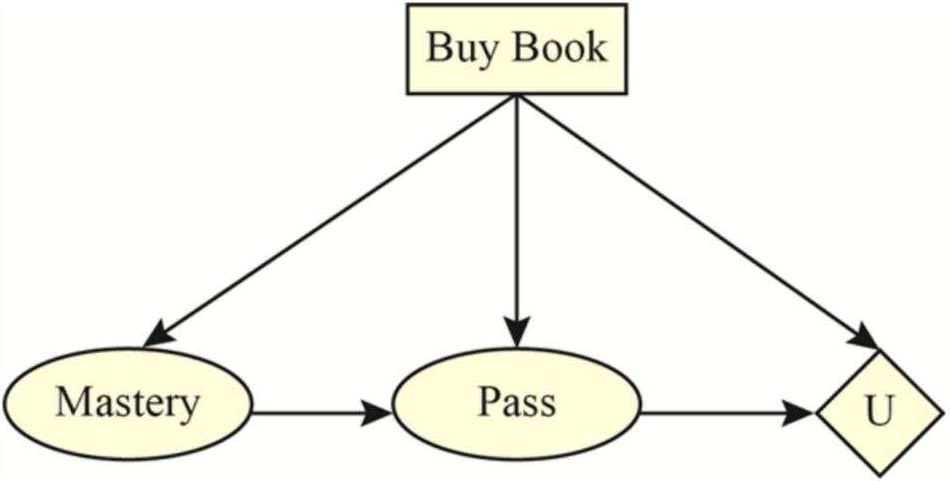
\includegraphics[width=0.45\textwidth]{pic1.png}
\end{figure}
It is a directed acyclic graph which has Buy Book as decision node, Mastery and Pass as chance node, and U as a utility node.
	\section*{\small Part 2}
The expected utility of buying the book is represented as EU[b] and not buying the book is represented by EU[$\neg b$]. They are computed as given below:
\begin{figure}[H]
	\centering
	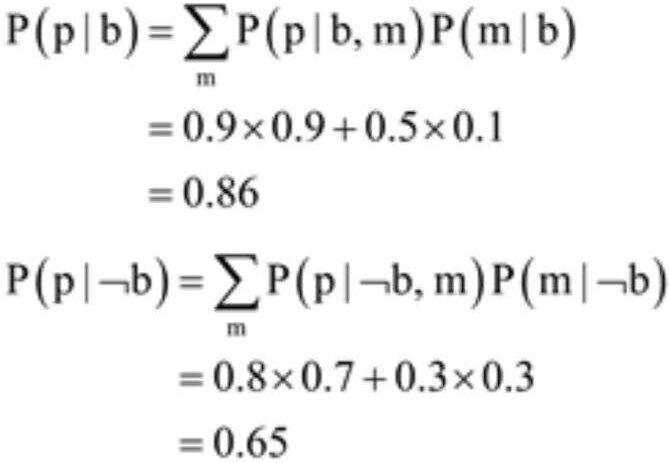
\includegraphics[width=0.28\textwidth]{pic2.png}
\end{figure}
So, the expected utility of buying the book is computed as:
\begin{figure}[H]
	\centering
	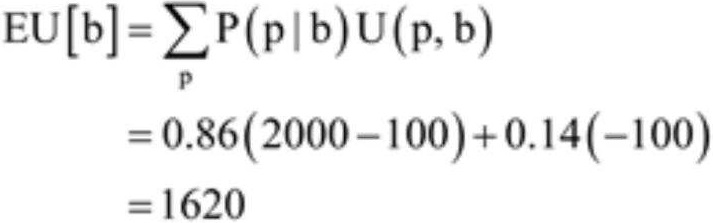
\includegraphics[width=0.3\textwidth]{pic3.png}
\end{figure}
The expected utility of not buying the book is computed as:
\begin{figure}[H]
	\centering
	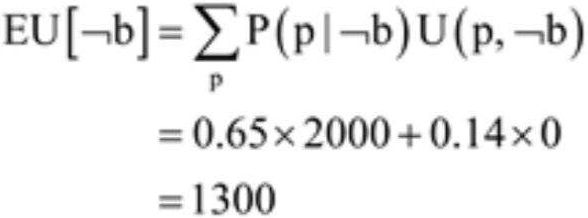
\includegraphics[width=0.26\textwidth]{pic4.png}
\end{figure}
	\section*{\small Part 3}
Since the expected utility of buying the book is less than not buying the book as the expected utility of buying the book is 1620 and the value 1620 is less than 1300 (expected utility of not buying the book), student should go for the option to purchase a book.
\end{solution}
\\\noindent\rule{7in}{2.8pt}
\pagebreak
%%%%%%%%%%%%%%%%%%%%%%%%%%%%%%%%%%%%%%%%%%%%%%%%%%%%%%%%%%%%%%%%%%%%%%%%%
\begin{problem}{4}
	
\end{problem}
\begin{solution}
 	\section*{\small Part 1}
 	\begin{figure}[H]
 		\centering
 		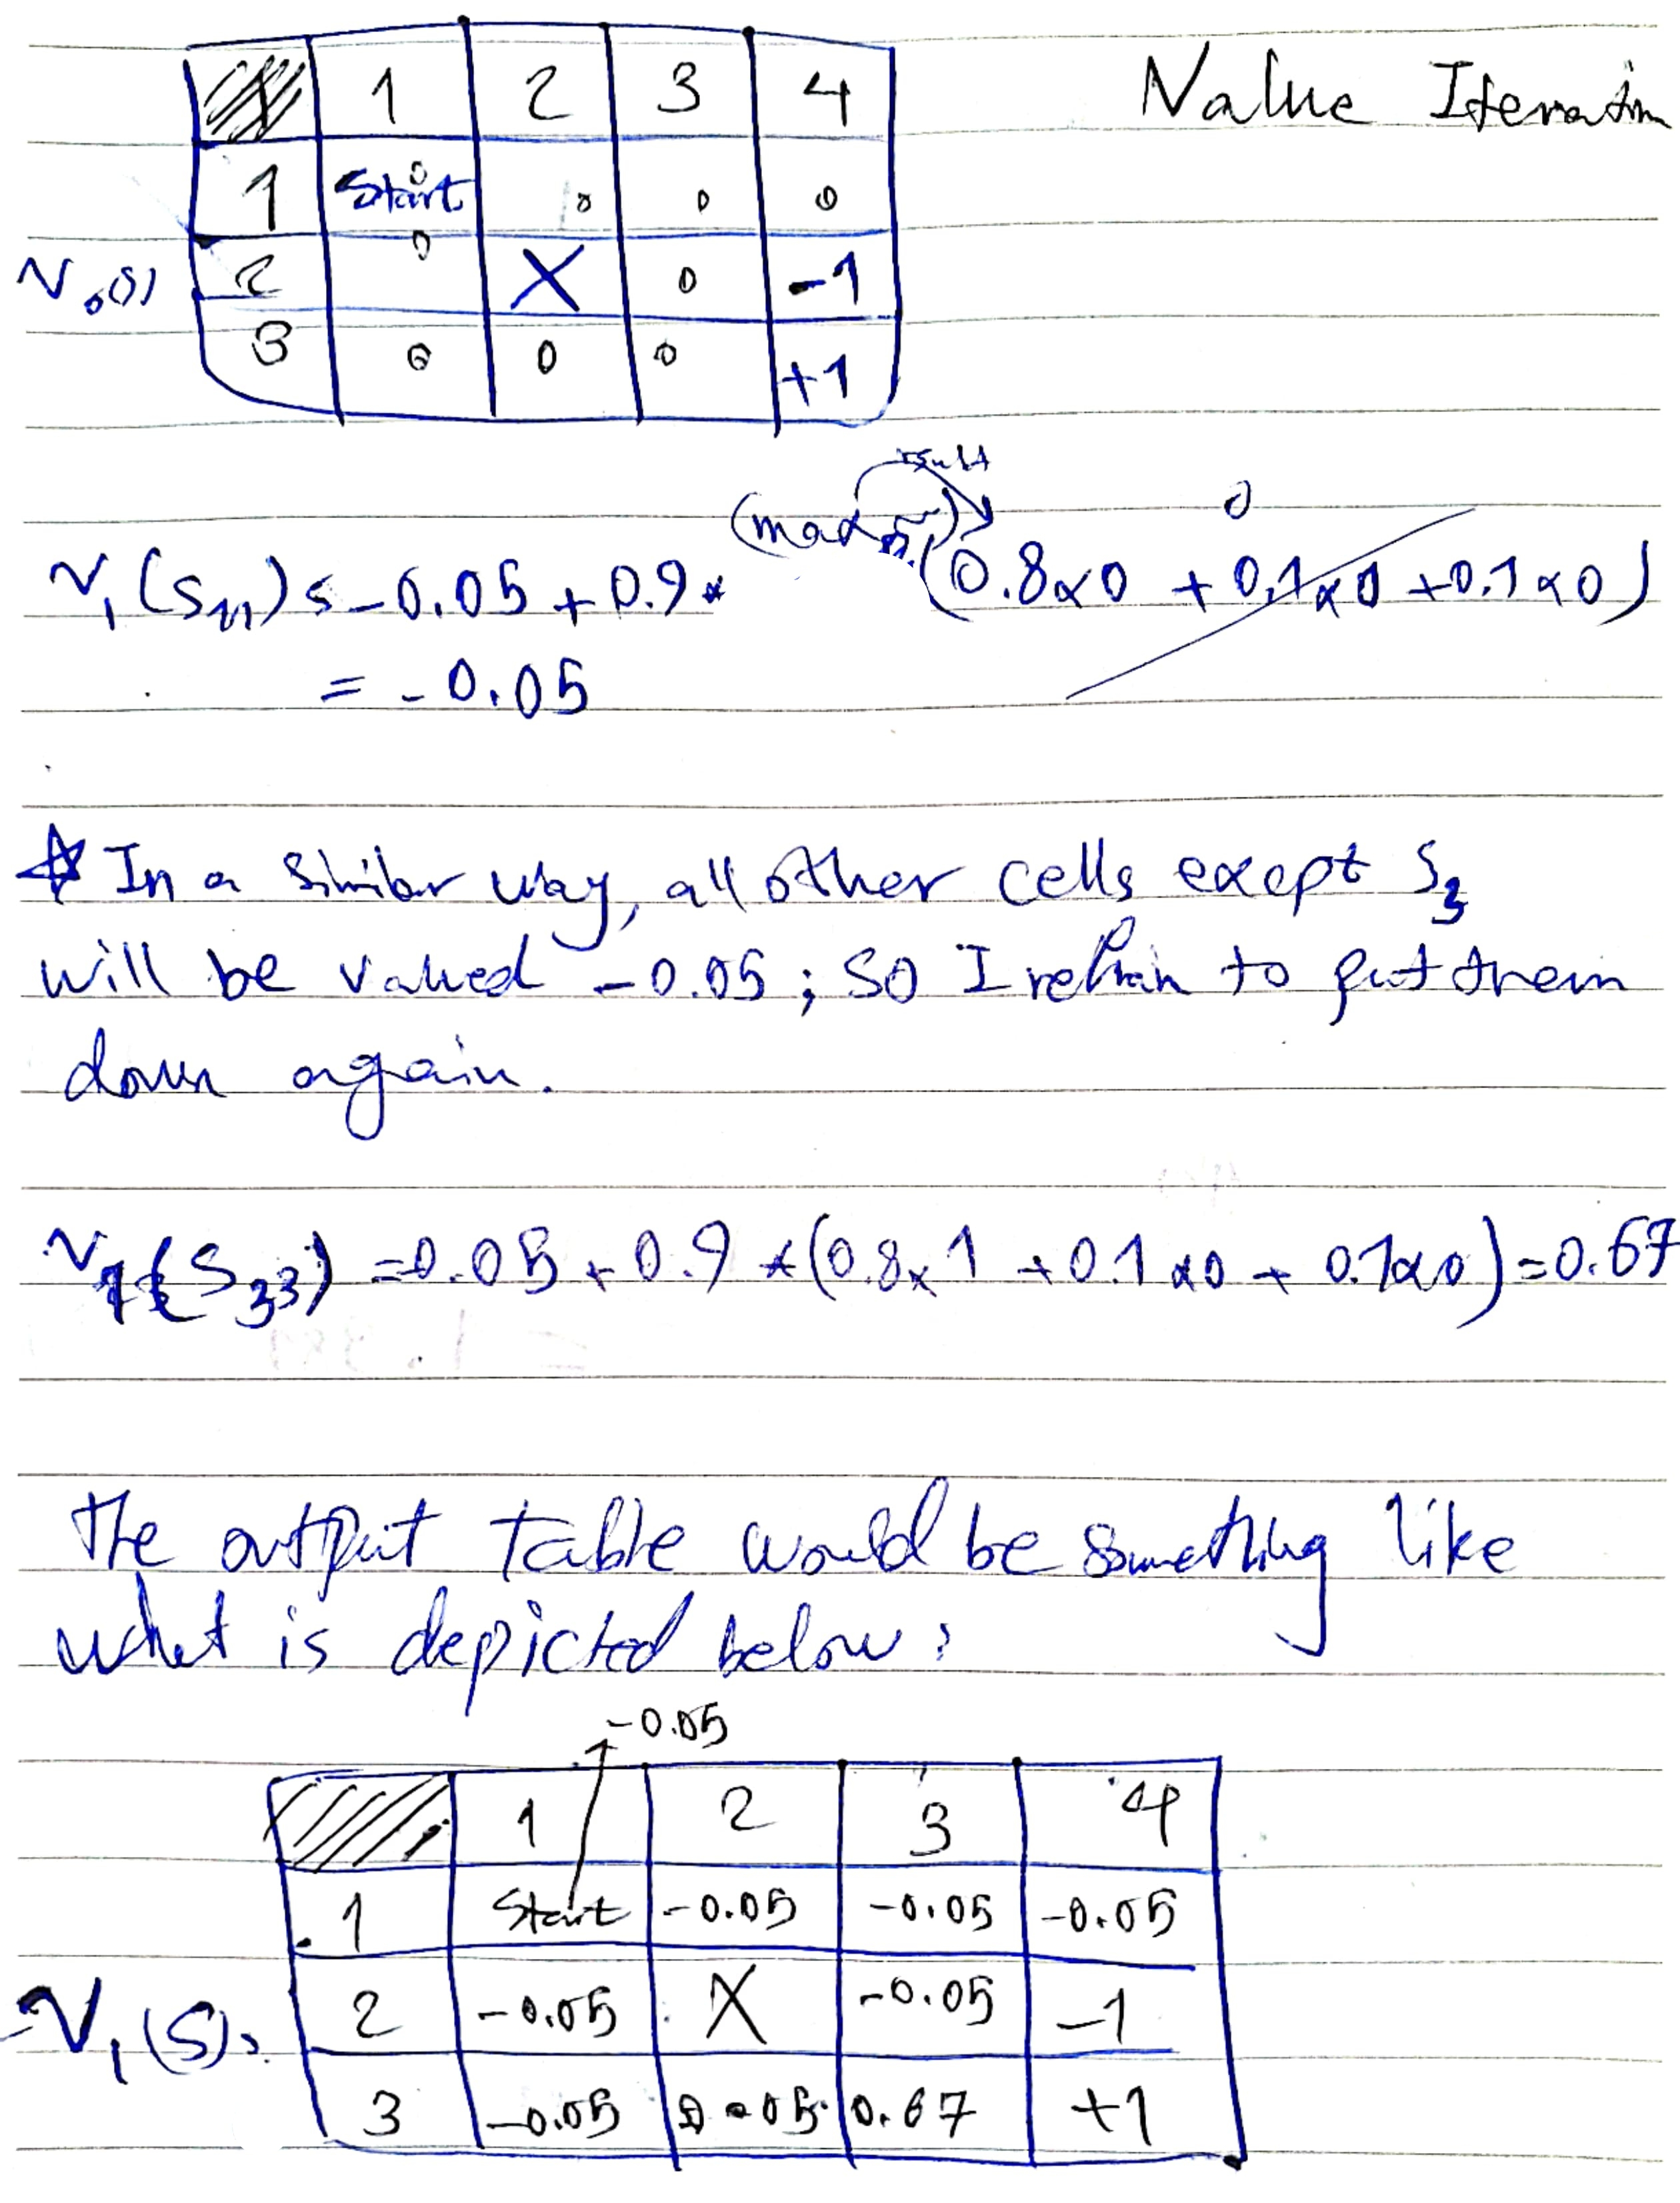
\includegraphics[width=0.9\textwidth]{1.jpg}
 	\end{figure}
 	\begin{figure}[H]
 		\centering
 		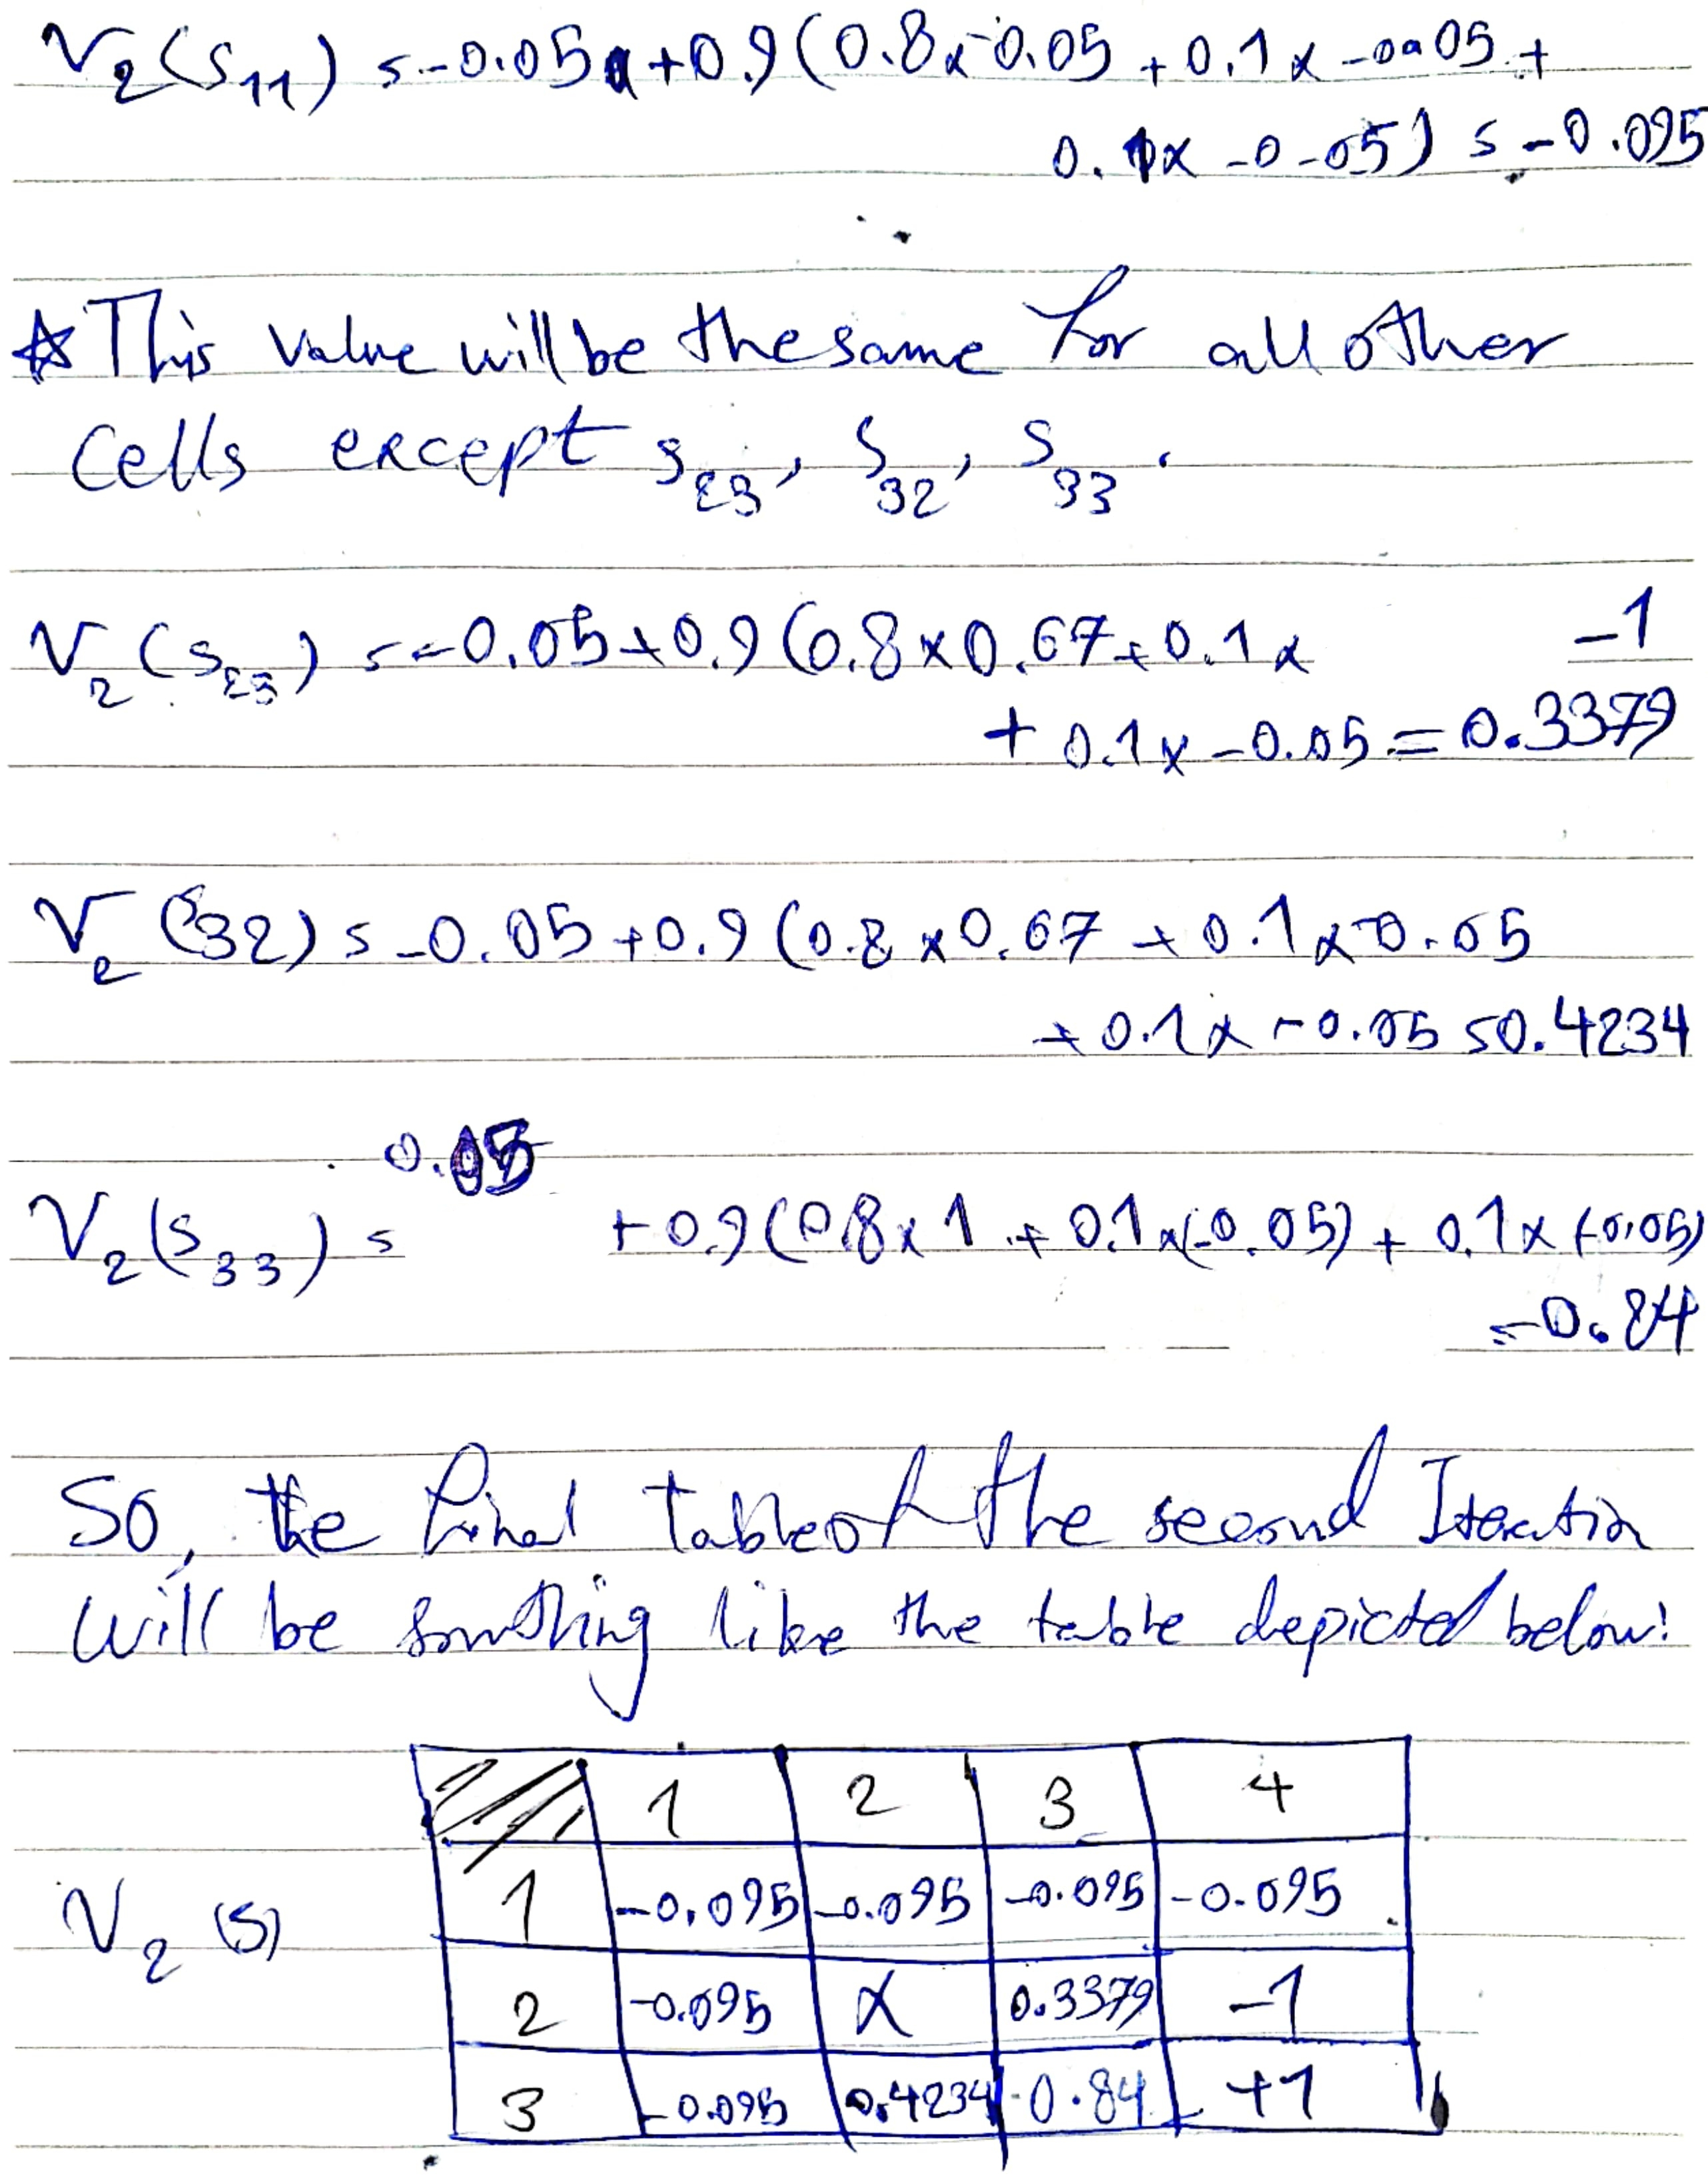
\includegraphics[width=0.9\textwidth]{2.jpg}
 	\end{figure}
 	 	\section*{\small Part 2}
 	\begin{figure}[H]
 		\centering
 		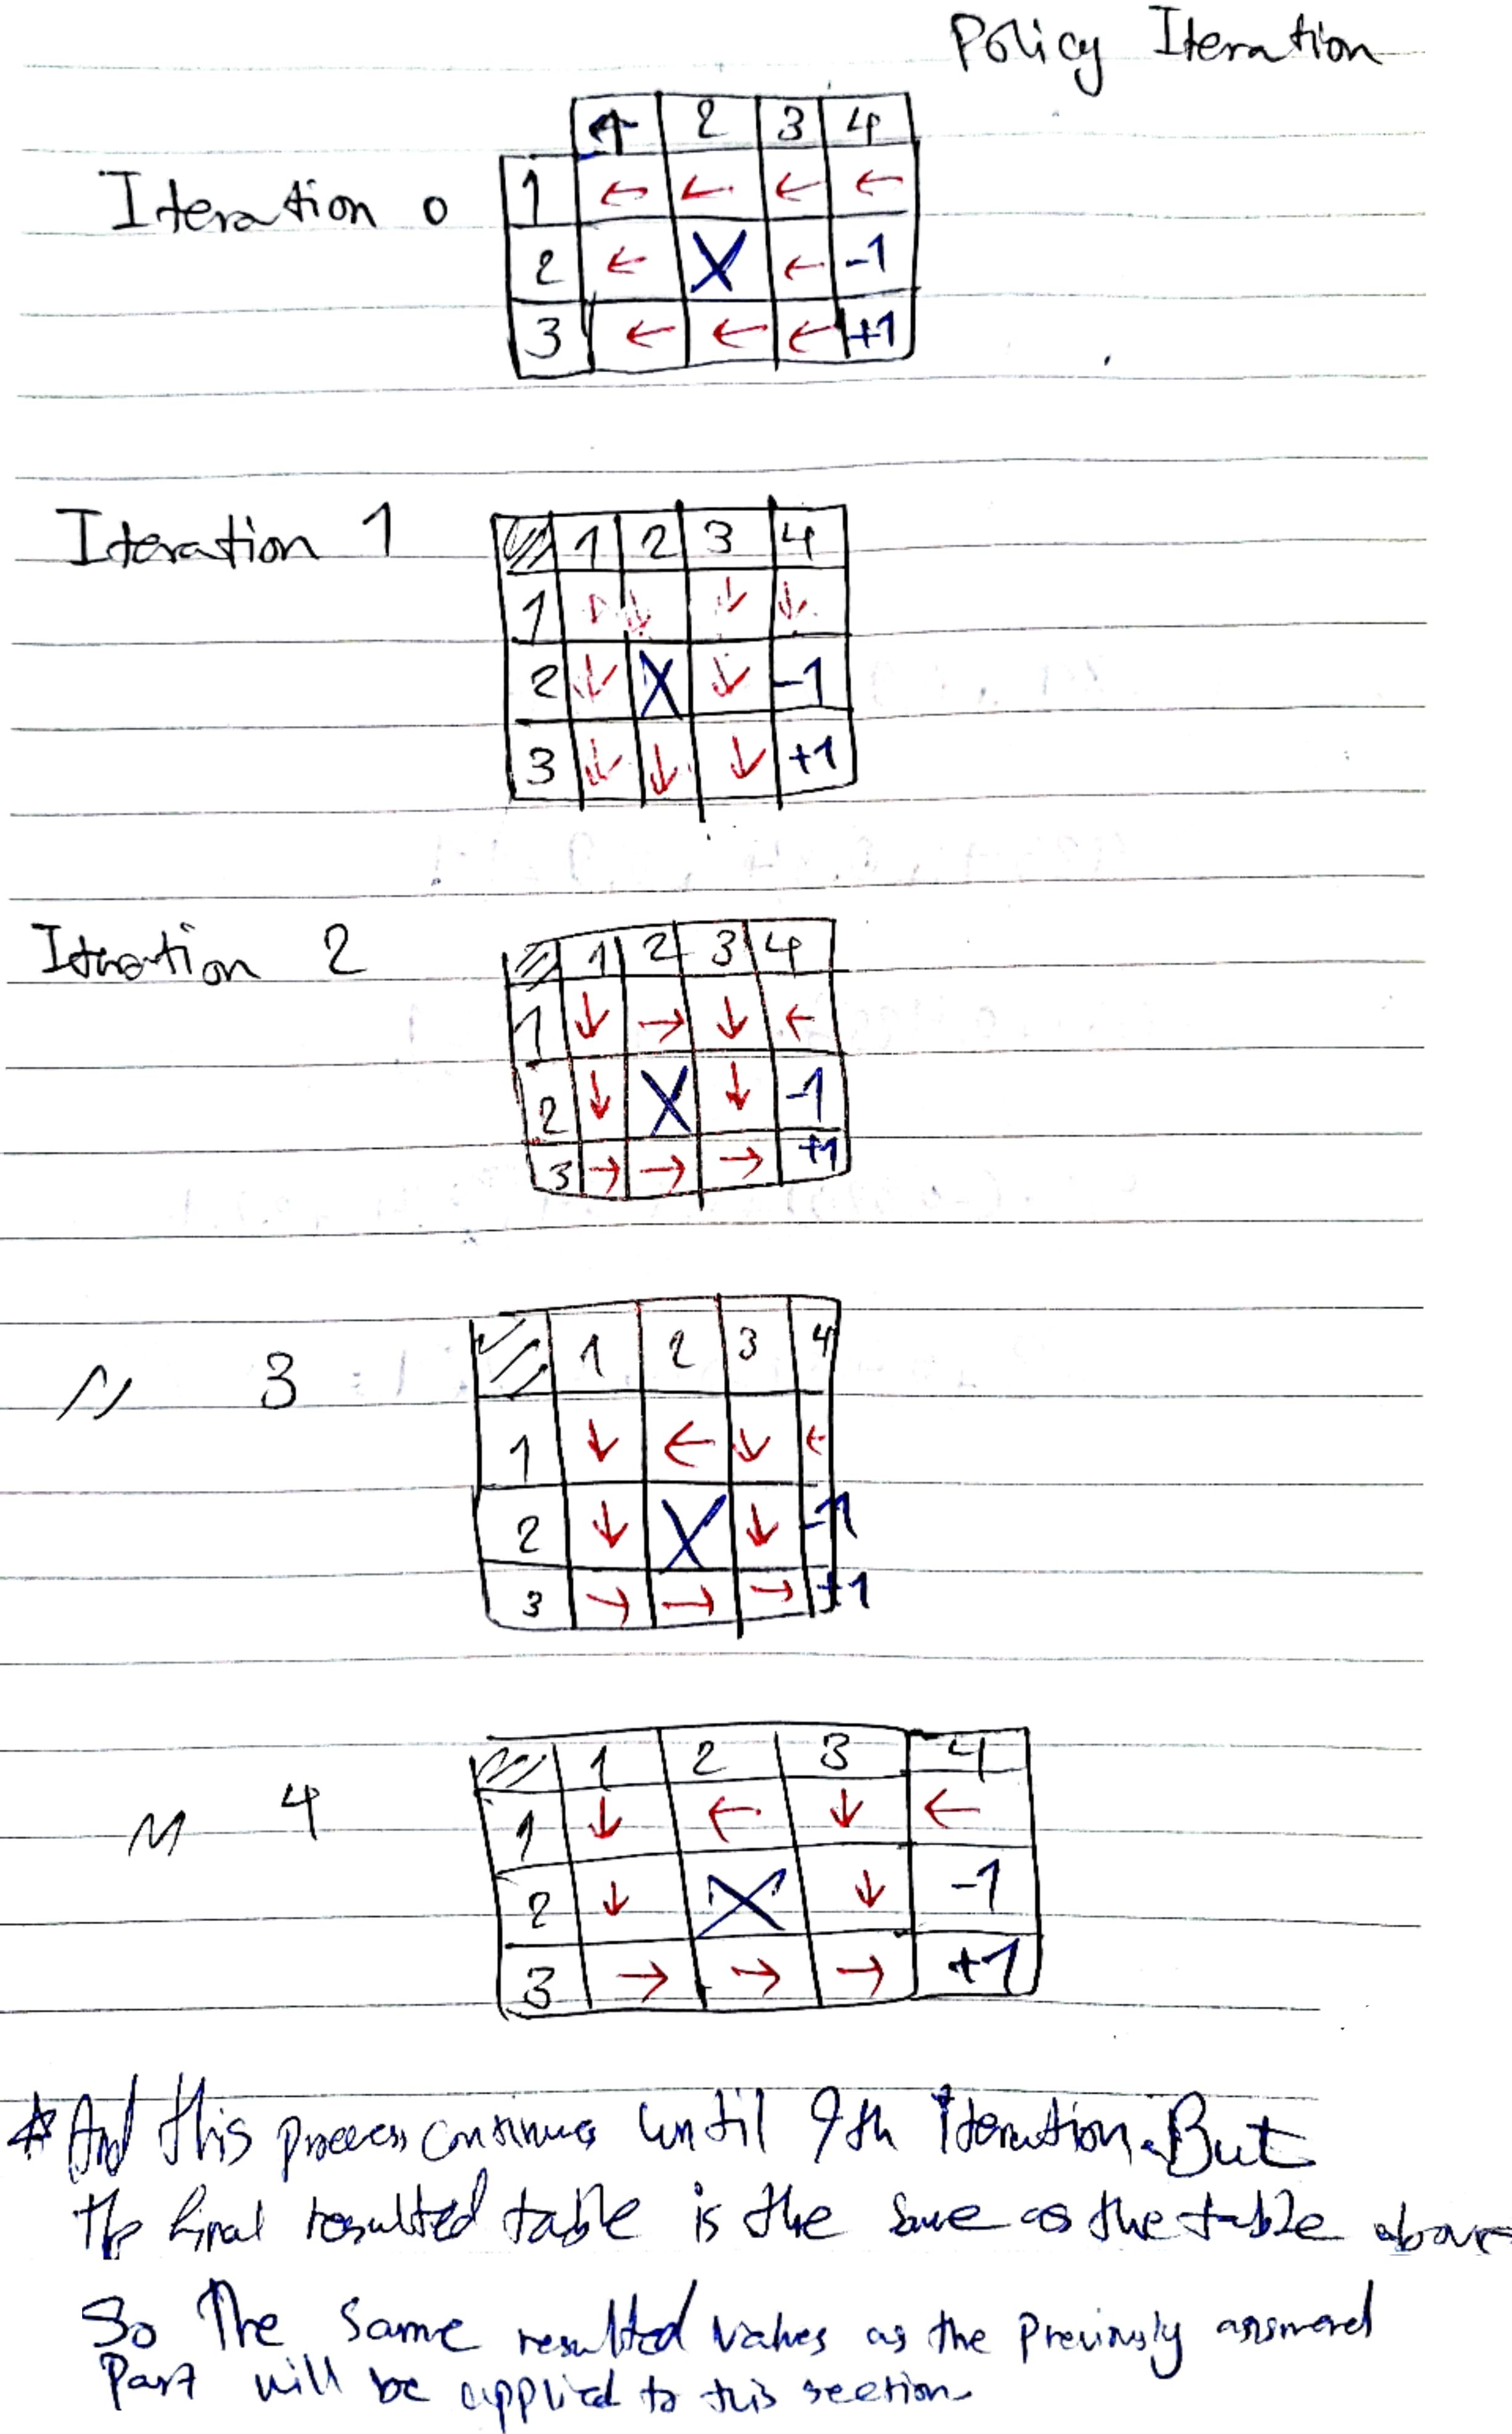
\includegraphics[width=0.85\textwidth]{3.jpg}
 	\end{figure}
 	 	 	\section*{\small Part 3}
 	\begin{figure}[H]
 		\centering
 		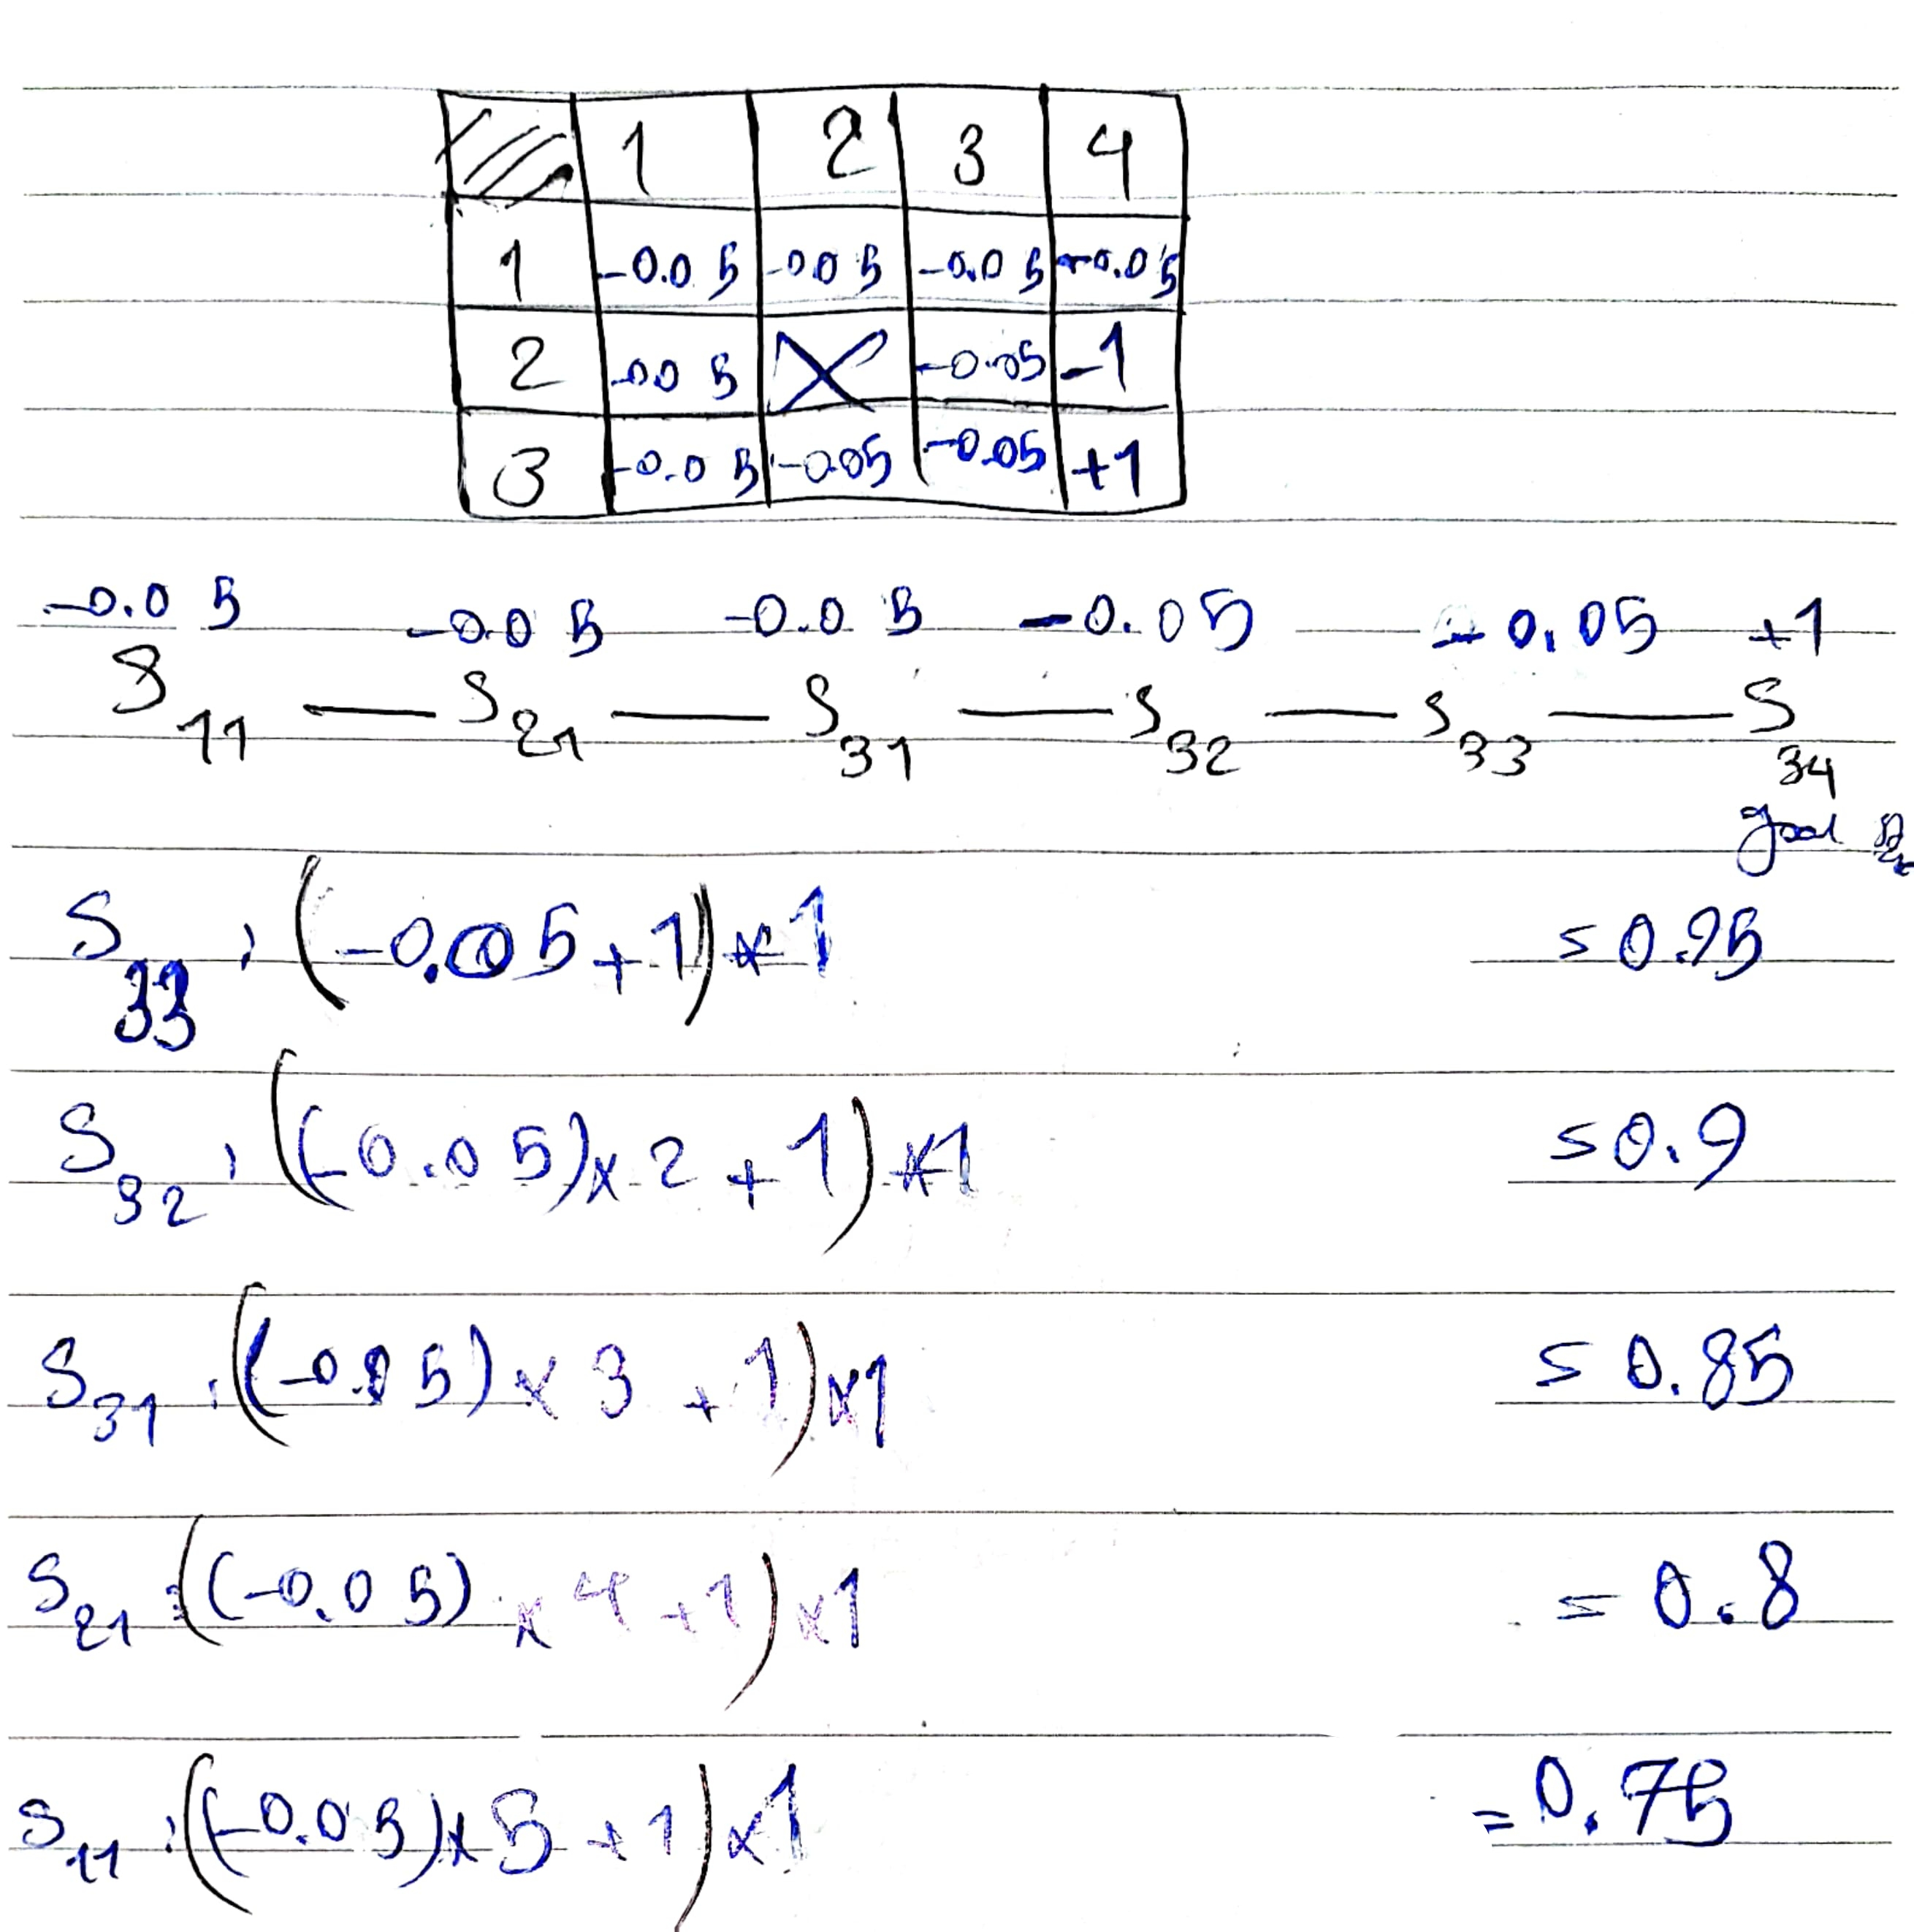
\includegraphics[width=0.9\textwidth]{4.jpg}
 	\end{figure}
\end{solution}
\noindent\rule{7in}{2.8pt}
\pagebreak
%%%%%%%%%%%%%%%%%%%%%%%%%%%%%%%%%%%%%%%%%%%%%%%%%%%%%%%%%%%%%%%%%%%%%%%%%
\end{document}
 